\documentclass[10pt, a4paper]{beamer} %handout fuer eine gedruckte version der slides
\usetheme{metropolis}

\usepackage{url}
\usepackage{polyglossia}
\setmainlanguage{english}

\usepackage{listings,xcolor}
\usepackage{graphicx}
\usepackage{nameref}

\makeatletter
\newcommand*{\currentname}{\@currentlabelname}
\makeatother

\usepackage{fontspec}
% \setmainfont{UbuntuMono}
\newfontfamily\Bera{Bitstream Vera Sans Mono}[Scale=0.85]

\definecolor{mDarkTeal}{HTML}{23373b}
\definecolor{mLightBrown}{HTML}{EB811B}
\definecolor{mDarkBlue}{HTML}{0F3470}
\definecolor{mDarkGrey}{HTML}{999999}
\definecolor{mLighterGrey}{HTML}{CCCCCC}
\definecolor{mLightGrey}{rgb}{0.95,0.95,0.95}

\setbeamercolor{block title}{fg=mDarkTeal}

\lstset{language=Python,
    backgroundcolor=\color{mLightGrey},
    frame=single,
    rulecolor=\color{mLightGrey}, % make frame "invisible"
    basicstyle=\Bera\footnotesize,
    keywordstyle=\bfseries\color{mDarkBlue},
    commentstyle=\color{mDarkGrey}\itshape,
    captionpos=t,
    emphstyle=\ttb\color{mDarkBlue},    % Custom highlighting style
    stringstyle=\color{mLightBrown},
    tabsize=2,
    numberbychapter=false,
    showstringspaces=false,
    breaklines=true,
    morekeywords={__init__, and, assert, break, class, continue, def, del, elif, else, except, exec, finally, for, from, global, if, import, in, is, lambda, not, or, pass, print, raise, return, try, while, yield}
}
%


\setbeamertemplate{section in toc}{%
  {\color{mDarkTeal}\rule[0.3ex]{3pt}{3pt}}~\inserttocsection\par}
\setbeamertemplate{subsection in toc}{%
  \hspace{1.2em}{\color{mLightBrown}\rule[0.3ex]{3pt}{3pt}}~\inserttocsubsection\par}


% \usecolortheme{spruce}
\AtBeginSection[]
{
  \begin{frame}
    \frametitle{\currentname}
    \tableofcontents[currentsection]
  \end{frame}
}

\AtBeginSubsection[]
{
  {
  \setbeamercolor{background canvas}{bg=mLighterGrey}
  \begin{frame}
    \frametitle{\currentname}
  \end{frame}
  }
}

\title % (optional, only for long titles)
{Foundations of Programming in Python}
\author % (optional, for multiple authors)
{Philipp Gloor\inst{1}}
\institute
{
  \inst{1}%
  University of Zurich
}
\date{}
\subject{Python}

\begin{document}
\begin{frame}
\titlepage
\end{frame}

\begin{frame}
\frametitle{About me}

\begin{block}{Education}
    \begin{itemize}
        \item 2012 -- Bachelor of Science UZH in Physics
        \item 2016 -- Master of Science UZH in Computational Science
    \end{itemize}
\end{block}

\begin{block}{Work}
    \begin{itemize}
        \item 2014 -- 2016 Software engineer CERN (remote)
        \item 2016 -- now PDF Tools AG
    \end{itemize}
\end{block}

\begin{block}{Programming experience}
    \begin{itemize}
        \item[] C++, C\#, Java, JavaScript, Python
    \end{itemize}
\end{block}

\begin{block}{Email}
\begin{itemize}
    \item[] philipp.gloor@gmail.com
\end{itemize}
    
\end{block}
 
% In this slide, some important text will be
% \alert{highlighted} beause it's important.
% Please, don't abuse it.
 
% \begin{block}{Remark}
% Sample text
% \end{block}
 
% \begin{alertblock}{Important theorem}
% Sample text in red box
% \end{alertblock}
 
% \begin{examples}
% Sample text in green box. "Examples" is fixed as block title.
% \end{examples}
\end{frame}
\begin{frame}[t]\frametitle{Round of introduction}
    \begin{itemize}
        \item Name
        \item Occupation
        \item Programming experience? What language?
        \item Expectations
    \end{itemize}
\end{frame}

\begin{frame}[t]\frametitle{Learning targets}
    
After this course...
\begin{itemize}
    \item ... you will know what programming is
    \item ... you will know how to write a basic computer program
    \item ... you will know the fundamental components of programming
    \item ... you are able to run Python code
    \item ... you are able to write a Python program based on a written out
    problem statement
    \item ... you know where you can find more information to improve your
    programming skills
\end{itemize}
\end{frame}


\section{Introduction to Programming} % (fold)
\label{sec:introduction_to_programming}

\begin{frame}[c]\frametitle{What is a Computer Program}
\begin{block}{Modular System}
    \begin{itemize}
        \item \textbf{Input}: Data input from keyboard, files, internet, etc...
        \item \textbf{Output}: Processed data is displayed or saved to a file
        \item \textbf{Assignment}: Values are assigned to variables
        \item \textbf{Conditional execution}: Statements are executed only if certain
        conditions are fulfilled
        \item \textbf{Loops}: Repeating statement or group of statements
        \item \textbf{Libraries}: Using existing implementations
    \end{itemize}

\end{block}     
\end{frame}

\begin{frame}[fragile,c,allowframebreaks]\frametitle{Examples: Hello World}
    \begin{block}{Java}
    {
    % \lstset
    \begin{lstlisting}[language=Java]
        public class HelloWorld {
            public static void main(String args[]) {
                System.out.println("Hello World");
            }
        }
    \end{lstlisting}    
    }
    \end{block}
    
    \begin{block}{C++}
    {
    % \lstset
    \begin{lstlisting}[language=C++, morekeywords=include]
        #include <iostream>
        int main() {
            std::cout << "Hello World" << std::endl;
            return 0;
        }
    \end{lstlisting}    
    }
    \end{block}
    \framebreak
    \begin{block}{Python}
        \begin{lstlisting}
            print("Hello World")
        \end{lstlisting}
    \end{block}
    
\end{frame}

\begin{frame}[c]\frametitle{Why Python?}
    \begin{columns}
        \begin{column}{0.5\textwidth}
           \begin{itemize}
                \item "Simple" syntax
                \item High-level programming language
                \item Cross-platform
                \item Interpreted
                \item Object-oriented
                \item Many libraries available
            \end{itemize}
        \end{column}
        \begin{column}{0.5\textwidth}  %%<--- here
            \begin{figure}
                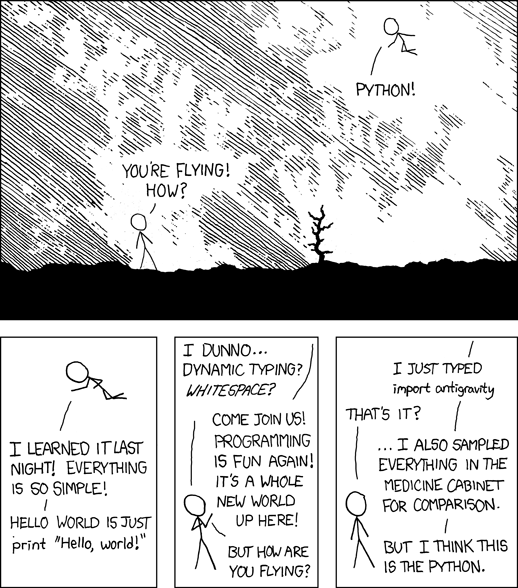
\includegraphics[width=0.9\linewidth]{pics/python.png}
            \end{figure}
            \tiny Source: https://xkcd.com/353/
        \end{column}
    \end{columns}

\end{frame}

\begin{frame}[c]\frametitle{Development Environment}

\begin{itemize}
    \item Integrated Development Environment (IDE)
    \item Collection of tools that are commonly used for software development
    \item Popular IDEs
    \begin{itemize}
        \item Eclipse with pydev - \url{http://pydev.org}
        \item JetBrains PyCharm - Community Edition available for free \url{http://jetbrains.com/pycharm/download}
    \end{itemize}
\end{itemize}
\end{frame}

\begin{frame}[fragile,c]\frametitle{Demo: Hello World}

\begin{block}{Options to run Python code:}
\begin{itemize}
    \item Directly in the Python prompt
    \item Write the code into a file and run python with the file
    \item Use IDE to run Python code
\end{itemize}



\end{block}
    
\end{frame}
% section introduction_to_programming (end)

\section{Fundamental Concepts} % (fold)
\label{sec:fundamental_concepts}

\subsection{Values, Variables, Expressions, Operators, Comments} % (fold)
\label{sub:values_variables_expressions_operators_comments}

\begin{frame}[c]\frametitle{Values, Variables, Expressions, Operators, Comments}
\begin{block}{Values}
    \begin{itemize}
        \item Numbers
        \begin{itemize}
            \item 2
            \item 1000000
            \item -2
            \item 3.2
            \item 1.3333333
        \end{itemize}
        \item Strings (Text)
        \begin{itemize}
            \item {\color{blue}'Hello World'}
            \item {\color{red}"Hello World"}
        \end{itemize}
    \end{itemize}
\end{block}
    
\end{frame}

\begin{frame}[c]\frametitle{Data Types}
    \begin{block}{Strings}
    \begin{itemize}
        \item {\color{blue} 'Single quotes'} or {\color{red} "double quotes"} can be used to declare them
        \begin{itemize}
            \item 'Hello World'
            \item "Hello World"
            \item "5"
        \end{itemize}
    \end{itemize}
    \end{block}
    \begin{block}{Boolean}
    Binary data type
        \begin{itemize}
            \item True
            \item False
        \end{itemize}
    \end{block}

\end{frame}

\begin{frame}[c,fragile,allowframebreaks]\frametitle{Variables}
    \begin{itemize}
        \item Variables hold values
        \item Similar to mathematics
        \begin{itemize}
            \item x = 2
            \item y = x + 2
        \end{itemize}
        \item Values assigned using the \texttt{=} operator
    \end{itemize}
    \begin{examples}
    Use meaningful names
    \begin{itemize}
        \item Declaration
        \begin{lstlisting}
            salutation = "Hello"
            name = "Dennis Reynolds"
            pi = 3.13159
        \end{lstlisting}
        \item Usage
        \begin{lstlisting}
            print(name)
        \end{lstlisting}
    \end{itemize}
        
    \end{examples}
\framebreak
\begin{block}{Keywords - reserved words}

\begin{lstlisting}
and, assert, break, class, continue, def, del, elif, else, except, exec, 
finally, for, from, global, if, import, in, is, lambda, not, or, pass, 
print, raise, return, try, while, yield
\end{lstlisting}
    
\end{block}
\framebreak
\begin{block}{Variables and values can be combined}
    \begin{lstlisting}
print(2+2)
a = 2
print(a+2)

salutation = "Hello"
name = "Dennis Reynolds"
print(salutation + " " + name)
    \end{lstlisting}
\end{block}
\end{frame}

\begin{frame}[t, fragile]\frametitle{Operators}
\begin{block}{Order of precedence}
\begin{itemize}
        \item ()
        \item **
        \item unary +,-
        \item *,/,\%
        \item binary +,-
        \item \texttt{<}, \texttt{>}, \texttt{<=}, \texttt{>=}, \texttt{!=}, \texttt{==}
        \item \textbf{\texttt{\color{mDarkBlue}not}}
        \item \textbf{\texttt{\color{mDarkBlue}and}}
        \item \textbf{\texttt{\color{mDarkBlue}or}}
    \end{itemize}    
\end{block}
    
\end{frame}

\begin{frame}[t, fragile]\frametitle{Comments}
\begin{itemize}
    \item Comments have no impact on the program
    \item Should explain the code
    \item A comment starts with a \# character
\end{itemize}

\begin{examples}
    \begin{lstlisting}
# Declaring the name
name = "Philipp"
print(name) # Prints Philipp
    \end{lstlisting}
\end{examples}
    


\end{frame}

% subsection values_variables_expressions_operators_comments (end)

\subsection{Functions} % (fold)
\label{sub:functions}
\begin{frame}[c, fragile,allowframebreaks]\frametitle{Functions}
\begin{itemize}
    \item \lstinline!print()! is a function that you have already used
    \item A function can take arguments which can be used inside the function
    \begin{lstlisting}
name = "Some name"
print(name) # Some name is used inside the print function
    \end{lstlisting}
    \item Functions can also return a result
    \begin{itemize}
        \item \lstinline!return! statement
    \end{itemize}
\end{itemize}

\begin{examples}
    \begin{lstlisting}
text = "Python programming language"
print(text) # Prints: Python programming language
text_length = len(text)
print(text_length) # Prints length of the string
    \end{lstlisting}
\end{examples}
\framebreak
\begin{block}{Type conversions}
\begin{itemize}
    \item \lstinline!int('32')!: Converts a string that holds a number to an integer
    \item \lstinline!int('Hello')!: This doesn't work and it will throw a ValueError exception
    \item \lstinline!float('313.333')!: Converts a string that hold a number to a float
    \item \lstinline!str(32)!: Converts a number to a string
\end{itemize}

\begin{examples}
\begin{lstlisting}
a = 20
b = 10
res = a + b
print("The sum of " + str(a) + " and " + str(b) + " is " + str(res))
\end{lstlisting}
\end{examples}
\end{block}

\framebreak

\begin{block}{Rounding}
    \begin{lstlisting}
a = 1.888
int(a) # = 1
int(round(a)) # = 2
int(a+5) # = 2
    \end{lstlisting}
\end{block}
\begin{block}{Math functions}
    \begin{lstlisting}
import math
log_res = math.log(17.0)
sin_res = math.sin(45)
angle = 20
x = math.cos(20*math.pi/180))  # cos/sin etc take radians as arguments -> conversion from degree to radians necessary      
    \end{lstlisting}
    \begin{itemize}
        \item \tiny \url{http://docs.python.org/library/math.html}
    \end{itemize}
\end{block}

\framebreak

\begin{block}{User-defined functions}
    \begin{itemize}
        \item A function encapsulates some functionality
        \item Reduces complexity
        \begin{lstlisting}
def my_function(param1, param2):
    print(param1)
    print(param2)            
        \end{lstlisting}
        \item Syntax is important
        \begin{itemize}
            \item Indentation
            \item The colon
        \end{itemize}
    \end{itemize}
\end{block}
\framebreak
\begin{examples}
    \begin{lstlisting}
def line_separator():
    print('')

print("First Line")
line_separator()
print("Second Line")
line_separator()
print("Third Line")
line_separator()
print("Fourth Line")
\end{lstlisting}
\end{examples}
\begin{itemize}
    \item If we want to change the line separator to a dashed line we only need to change a single line of code
\end{itemize}
\begin{lstlisting}
def line_separator():
print('------------------------------')
\end{lstlisting}


\framebreak

\begin{examples}
    \begin{itemize}
        \item If the line seperator should output two lines we can define a new function that calls the \lstinline!line_separator()! function twice
    \end{itemize}
    \begin{lstlisting}
def two_lines():
    line_separator()
    line_separator()

print ("First Line")
two_lines()
print("Second Line")       
    \end{lstlisting}
\end{examples}

\framebreak
\begin{block}{Parameters and arguments}
    \begin{itemize}
        \item Arguments are passed when calling a function
        \item Value of arguments is assigned to parameters
    \end{itemize}
    \begin{lstlisting}
def print_sum(number_1, number_2):
    result = number_1 + number_2
    print(result)

print_sum(1,3)
print_sum(10,5)
    \end{lstlisting}
\end{block}
\begin{block}{Parameters and arguments}
    \framebreak
    \begin{itemize}
        \item Variables are valid within a scope
        \item Variables that are defined in a function can only be seen inside that function
        \item Scope can be identified by indentation
    \end{itemize}
    \begin{lstlisting}
def concatenation(param1, param2):
    concat = part1 + part2
    print(concat)

concatenation("Hello", "World")
print(concat) # NameError: name 'concat' is not defined
    \end{lstlisting}
\end{block}
\begin{block}{Conclusion}
    \begin{itemize}
        \item A function can be called multiple times
        \item If some code can be reused, put it in a function so you need to write less
        \begin{itemize}
            \item Higher factorization
            \item Less redundancy
            \item Better maintenance
        \end{itemize}
        \item Functions can also call other functions
    \end{itemize}
\end{block}
\end{frame}
% subsection functions (end)

\subsection{Naming Conventions \& Debugging} % (fold)
\label{sub:naming_conventions_&_debugging}
\begin{frame}[c,fragile, allowframebreaks]\frametitle{Naming Conventions}
\begin{block}{How to name your functions and variables (PEP8)}
    \begin{itemize}
\item Naming convention is a set of rules for choosing names of functions and variables
\item Every programming language has different naming conventions
\item Python
\begin{itemize}
    \item No spaces in variable and function names
    \item Variable and function names are in lowercase and \_ is used to separate words
\end{itemize}
    \end{itemize}

\begin{lstlisting}
length_in_cm = 15

def say_hello():
    print("Hello")    
\end{lstlisting}
\end{block}
\end{frame}

\begin{frame}[c,allowframebreaks]\frametitle{Debugging}
\begin{block}{Finding and resolving "bugs"}
\begin{itemize}
\item Programming is a complex activity
\item Mistakes happen all the time
\item A mistake made in programming is called a bug
\item The process of finding and resolving bugs is called debugging
\end{itemize}
\end{block}

\begin{block}{Errors}
    \begin{itemize}
        \item Syntax error
        \begin{itemize}
            \item Incorrect syntax of a statement: \lstinline!print(Hello World)! instead of \lstinline!print("Hello World")!
        \end{itemize}
        \item Runtime error
    
    \begin{itemize}
        \item Error that occurs during the execution of a program
        \item e.g. division by 0
    \end{itemize}
        \item Semantic errors
        \begin{itemize}
            \item Program does not deliver correct results
            \item No error messages (code is syntactically correct)
            \item Fixing semantic errors can be extremely complicated (good software design is important)
        \end{itemize}
    \end{itemize}
\end{block}
\framebreak
\begin{block}{Techniques}
\begin{itemize}
        \item Reading code
        \item Print variables with \lstinline!print()! to examine values (a poor man's debugger)
        \item Go through the program step by step -> \textbf{Debugger}!
    \end{itemize}    
\end{block}
    


\end{frame}
% subsection naming_conventions_&_debugging (end)

\subsection{Conditionals} % (fold)
\label{sub:conditionals}

\begin{frame}[c,fragile, allowframebreaks]\frametitle{Conditionals}
\begin{itemize}
\item Boolean algebra is a part of mathematics
\item Often used in programming
\item A boolean expression is either true or false
\end{itemize}

\begin{lstlisting}
5 == 5 # --> True
5 == 6 # --> False
6 > 4 # --> True
5 >= 8 # --> False
\end{lstlisting}

\framebreak
{
    \footnotesize

\begin{examples}

    \begin{block}{\color{mLightBrown}if}

        \begin{itemize}
            \item The expression if defines a condition
            \item If the condition is true, subsequent statements will be executed
            \item If the condition is false, subsequent statements will not be executed
            \item There has to be at least one statement after the condition
        \end{itemize}

    \end{block}
\end{examples}

\begin{lstlisting}
x = 10
if x > 0:
    print(str(x) + ' is positive')
if True:
    # This statement will always be executed
    print('Yes')
if False:
    # This statement will never be executed
    print('No')
\end{lstlisting}
}
\framebreak

    \begin{block}{\color{mLightBrown}else}
        \begin{itemize}
        \item Expression else is executed if the if condition is false
        \item Can only be used in combination with an if expression            
        \end{itemize}
    \end{block}

\begin{lstlisting}
if x == 0:
    print(str(x) + ' is zero')
else:
    print(str(x) + ' is not zero')
\end{lstlisting}

\framebreak

\begin{examples}
    \begin{block}{\color{mLightBrown}\%-operator (remainder after division)}
    {}
    \end{block}
\end{examples}
\begin{lstlisting}
def print_parity(x):
if x % 2 == 0:
    print(str(x) + ' is even')
else:
    print(str(x) + ' is odd')

print_parity(2)
print_parity(3)
\end{lstlisting}

\end{frame}
% subsection conditionals (end)

\subsection{Functions with Return Values} % (fold)
\label{sub:functions_with_return_values}

% subsection functions_with_return_values (end)

\subsection{Lists} % (fold)
\label{sub:lists}

% subsection lists (end)

\subsection{Iteration} % (fold)
\label{sub:iteration}

% subsection iteration (end)

\subsection{Dictionaries} % (fold)
\label{sub:dictionaries}

% subsection dictionaries (end)
% section fundamental_concepts (end)

\section{Persistence} % (fold)
\label{sec:persistence}

% section persistence (end)

\end{document}
